\documentclass[]{article}
\usepackage{lmodern}
\usepackage{amssymb,amsmath}
\usepackage{ifxetex,ifluatex}
\usepackage{fixltx2e} % provides \textsubscript
\ifnum 0\ifxetex 1\fi\ifluatex 1\fi=0 % if pdftex
  \usepackage[T1]{fontenc}
  \usepackage[utf8]{inputenc}
\else % if luatex or xelatex
  \ifxetex
    \usepackage{mathspec}
  \else
    \usepackage{fontspec}
  \fi
  \defaultfontfeatures{Ligatures=TeX,Scale=MatchLowercase}
\fi
% use upquote if available, for straight quotes in verbatim environments
\IfFileExists{upquote.sty}{\usepackage{upquote}}{}
% use microtype if available
\IfFileExists{microtype.sty}{%
\usepackage{microtype}
\UseMicrotypeSet[protrusion]{basicmath} % disable protrusion for tt fonts
}{}
\usepackage[margin=1in]{geometry}
\usepackage{hyperref}
\hypersetup{unicode=true,
            pdftitle={Hurricane Maria Mortality Study FAQ},
            pdfborder={0 0 0},
            breaklinks=true}
\urlstyle{same}  % don't use monospace font for urls
\usepackage{graphicx,grffile}
\makeatletter
\def\maxwidth{\ifdim\Gin@nat@width>\linewidth\linewidth\else\Gin@nat@width\fi}
\def\maxheight{\ifdim\Gin@nat@height>\textheight\textheight\else\Gin@nat@height\fi}
\makeatother
% Scale images if necessary, so that they will not overflow the page
% margins by default, and it is still possible to overwrite the defaults
% using explicit options in \includegraphics[width, height, ...]{}
\setkeys{Gin}{width=\maxwidth,height=\maxheight,keepaspectratio}
\IfFileExists{parskip.sty}{%
\usepackage{parskip}
}{% else
\setlength{\parindent}{0pt}
\setlength{\parskip}{6pt plus 2pt minus 1pt}
}
\setlength{\emergencystretch}{3em}  % prevent overfull lines
\providecommand{\tightlist}{%
  \setlength{\itemsep}{0pt}\setlength{\parskip}{0pt}}
\setcounter{secnumdepth}{0}
% Redefines (sub)paragraphs to behave more like sections
\ifx\paragraph\undefined\else
\let\oldparagraph\paragraph
\renewcommand{\paragraph}[1]{\oldparagraph{#1}\mbox{}}
\fi
\ifx\subparagraph\undefined\else
\let\oldsubparagraph\subparagraph
\renewcommand{\subparagraph}[1]{\oldsubparagraph{#1}\mbox{}}
\fi

%%% Use protect on footnotes to avoid problems with footnotes in titles
\let\rmarkdownfootnote\footnote%
\def\footnote{\protect\rmarkdownfootnote}

%%% Change title format to be more compact
\usepackage{titling}

% Create subtitle command for use in maketitle
\newcommand{\subtitle}[1]{
  \posttitle{
    \begin{center}\large#1\end{center}
    }
}

\setlength{\droptitle}{-2em}
  \title{Hurricane Maria Mortality Study FAQ}
  \pretitle{\vspace{\droptitle}\centering\huge}
  \posttitle{\par}
  \author{}
  \preauthor{}\postauthor{}
  \date{}
  \predate{}\postdate{}


\begin{document}
\maketitle

Hurricane Maria Mortality Study (NEJM online, Kishore et al., May 29
2018)

Available online:
\url{https://www.nejm.org/doi/full/10.1056/NEJMsa1803972}

Last updated: May 31, 2018

\subsection{FAQs}\label{faqs}

In response to the overwhelming media response and inquiries, the
authors have prepared this document to answer frequently asked
questions.

\subsection{What is the bottom line?}\label{what-is-the-bottom-line}

\begin{itemize}
\tightlist
\item
  We estimated that the mortality rate (the number of deaths per 1000
  people per unit time) remained high for months after the hurricane.
  This suggests that people continued to suffer even after the hurricane
  passed.
\item
  Our data suggests that about one third of those that died after the
  hurricane died from delayed or interrupted medical care, as reported
  by the surveyed households.
\item
  Even the low-bound of our estimates is consistent with earlier
  academic and press reports about the high mortality rate.
\item
  We intentionally used a simple method, but there are many ways to
  calculate excess deaths. We have made all data available and welcome
  other researchers’ analyses.
\end{itemize}

\subsection{How many people died?}\label{how-many-people-died}

We do not know exactly how many people died. Our estimates are based on
a household survey, where we visited 3299 randomly selected houses
across the island. Because the survey is based on a random sample, there
is uncertainty associated with our estimate. Our analysis suggests that
between 793 and 8498 people died after the hurricane and up to the end
of 2017, either directly or indirectly due to the hurricane.

\subsection{Does your study say that 4645
died?}\label{does-your-study-say-that-4645-died}

No. We provide a 95\% confidence interval of 793 to 8498, and 4645 falls
in the middle of this range.

\subsection{What is a confidence
interval?}\label{what-is-a-confidence-interval}

We implemented an approach that generates a confidence interval that has
a 95\% chance of including the actual death count. We followed a
standard statistical approach to calculate this interval. Our estimate
is based on a random sample of the entire population. If we took a
different random sample, and followed the same statistical approach, we
would end up with a different interval due to random variability
introduced by the sampling — because we would end up picking a
different set of households. If one had unlimited resources, and
continued to take random samples, 95\% of the resulting confidence
intervals would include the actual death count. All this requires
certain assumptions to hold; some are described in our paper, others
described in basic statistics textbooks.

\subsection{Why is your confidence interval so
large?}\label{why-is-your-confidence-interval-so-large}

Deaths are relatively rare events. We were able to survey 3299
households and found 56 deaths for the whole year (18 before the
hurricane, 38 after the hurricane). Since this number is small, when we
extrapolate the rate that we calculate from our survey up to the whole
population of Puerto Rico, we cannot be precise. To narrow the
confidence interval, one would need to survey an even larger numbers of
households.

\subsection{Why do you provide two confidence
intervals?}\label{why-do-you-provide-two-confidence-intervals}

The first interval, 793 to 8498, is based on the raw rate. We noted that
our survey was unable to capture the deaths of people that lived alone.
The paper describes an attempt to adjust for this “bias” and we
provide the confidence interval, 1506 to 9889, that is obtained after
this adjustment.

\begin{figure}
\centering
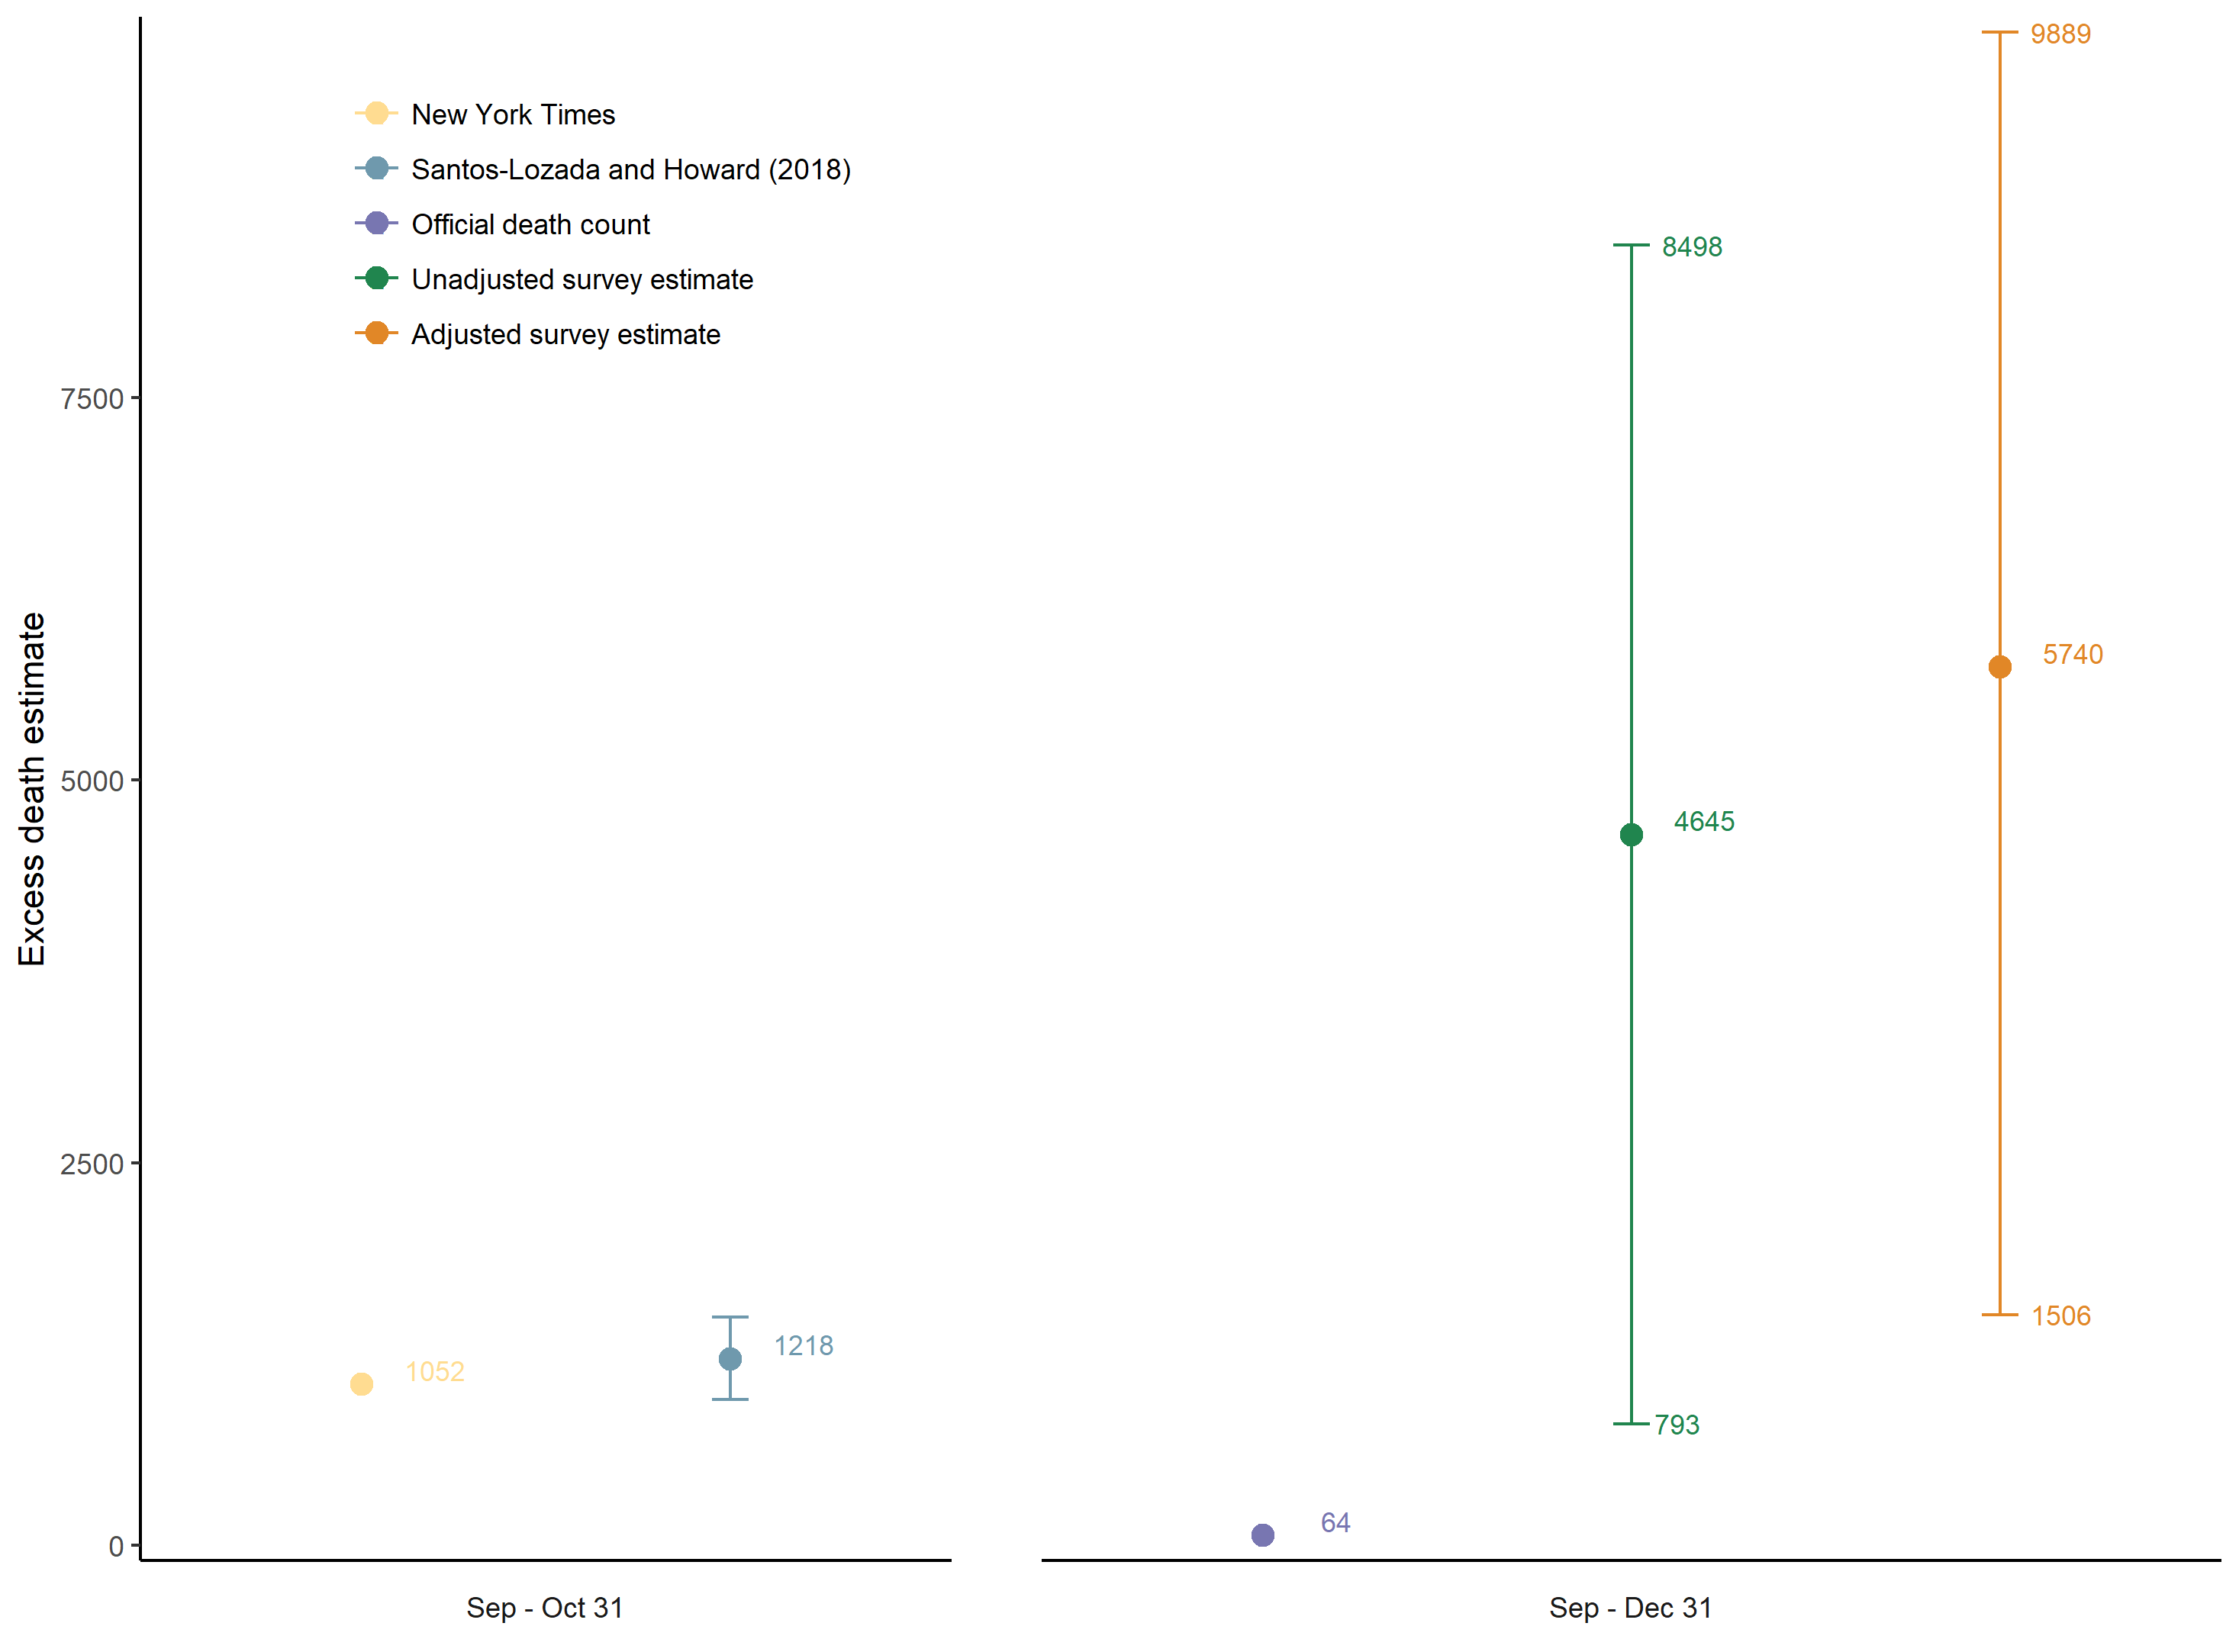
\includegraphics{../misc/faq_fig.png}
\caption{Figure 4a from the manuscript with labels added for the
confidence intervals}
\end{figure}

\subsection{What does a household-based survey
mean?}\label{what-does-a-household-based-survey-mean}

We picked a representative random sample of households from across
Puerto Rico. We divided all barrios in Puerto Rico into eight groups,
based on how urban or remote they were, and randomly selected
neighborhoods from each group. From each of the 104 selected
neighborhoods, we then again randomly selected about 35 households per
neighborhood. Additional details are discussed in the Supplement of our
paper accessible here:
\url{https://www.nejm.org/doi/suppl/10.1056/NEJMsa1803972/suppl_file/nejmsa1803972_appendix.pdf}

\subsection{Is this a new way to count
deaths?}\label{is-this-a-new-way-to-count-deaths}

No, household based surveys for estimating mortality after disasters are
a well established practice, and extensively described in the scientific
literature. Our paper cites several such studies. It is a cost-effective
and complementary way to count deaths.

\subsection{What does excess deaths
mean?}\label{what-does-excess-deaths-mean}

Excess deaths refers to the total number of deaths that exceeded the
number one would expect in “normal” years over the same time period.
This includes deaths from all causes. We compared our calculated the
mortality rate to that in the same period in 2016 to account for
seasonal variation. We also looked at the preceding six years, and found
that the death rate remained mostly stable in prior years. See Figure S2
of our Supplement, accessible here:
\url{https://www.nejm.org/doi/suppl/10.1056/NEJMsa1803972/suppl_file/nejmsa1803972_appendix.pdf}

\subsection{What are the names of the people that died? Why can’t you
tell
us?}\label{what-are-the-names-of-the-people-that-died-why-canat-you-tell-us}

It is standard practice to de-identify data before analysis to protect
the identity of respondents. It is also a precondition to our study
protocol being approved by the IRB (the ethics review board of the
Harvard Chan school). This is the norm is such studies, and considered
good and necessary practice to protect individuals from harm.

\subsection{What would you do differently if you can to do it
again?}\label{what-would-you-do-differently-if-you-can-to-do-it-again}

This was a quick study on a limited budget. With more time and
resources, we would recommend a larger sample size in order to narrow
the range of estimates.

\subsection{Why didn't you use the Demographic Registry data as done by
others?}\label{why-didnt-you-use-the-demographic-registry-data-as-done-by-others}

The government stopped sharing these data once they made a decision to
reevaluate the death toll.

\subsection{Who conducted this study? Were there Puerto Ricans on your
team?}\label{who-conducted-this-study-were-there-puerto-ricans-on-your-team}

This study was conducted by researchers and graduate students from
Harvard University (the FXB Center for Health and Human Rights, the
Epidemiology Department, Dana Farber Cancer Institute Department of
Biostatistics and Computational Biology, the Beth Israel Deaconess
Medical Center Emergency Department), Carlos Albizu University, Ponce
University, Puerto Rico Science and Research Trust, and the University
of Colorado Department of Emergency Medicine. A team of 50 graduate
students from Albizu and Ponce universities conducted the field
interviews, supervised by local faculty.

\subsection{What is the difference between this study and the study
commissioned by the Government of Puerto
Rico?}\label{what-is-the-difference-between-this-study-and-the-study-commissioned-by-the-government-of-puerto-rico}

The government has acknowledged that the official estimate is probably
low. As a result, they have commissioned a re-evaluation of individual
death certificate data, which will provide a detailed number based on
the death registry. Our study was completely independent of the death
registry data and provides different but complementary data about
deaths, as well as information about access to medical services and
utilities, and population displacement caused by the hurricane.

\subsection{Why did you conduct this study if GWU was doing
theirs?}\label{why-did-you-conduct-this-study-if-gwu-was-doing-theirs}

The study was underway when the announcement was made. Our methods are
different from the detailed recount that will be undertaken by GWU, and
will complement theirs and other approaches. To aid all researchers, and
in the spirit of complete transparency we have made all our data
available online.

\subsection{More information}\label{more-information}

We are unable to answer additional press inquiries by phone. For
interviews, please contact:
\href{mailto:tdatz@hsph.harvard.edu}{\nolinkurl{tdatz@hsph.harvard.edu}}

For statistical queries, please contact the corresponding author.
\url{https://www.nejm.org/doi/full/10.1056/NEJMsa1803972}


\end{document}
